\documentclass{article}

\usepackage[utf8]{inputenc}
\usepackage[german]{babel}
\usepackage[
    a4paper, top=2.5cm, bottom=2.5cm, left=2.5cm, right=2.5cm, marginparwidth=1.75cm
]{geometry}
\usepackage{amsmath}
\usepackage{amsfonts}
\usepackage{enumitem}
\usepackage[
    colorlinks=true, 
    citecolor=black,
    filecolor=black,
    linkcolor=black,
    urlcolor=blue
]{hyperref}
\usepackage{graphicx}
\usepackage{multirow}
\usepackage{amssymb}
\usepackage{float}
\usepackage{siunitx} \sisetup{locale = DE, uncertainty-mode = separate}
\usepackage{pdfpages}
\usepackage{multirow}
\usepackage[
    tocskip=0.1\baselineskip, skip=0.7\baselineskip, parfill
]{parskip}
\usepackage{listings}
\usepackage{fancyhdr}
\usepackage{xcolor}

% Kopf- und Fußzeile
\pagestyle{fancy}
\fancyhf{}
%Kopfzeile mittig mit Kaptilname
\fancyhead[C]{\nouppercase{\leftmark}}
%Fußzeile links bzw. innen
\fancyfoot[L]{\versuchsname}
%Fußzeile mittig (Seitennummer)
\fancyfoot[R]{\thepage}
\renewcommand{\footrulewidth}{0.35pt}

% Hilfs-Commands für Gleichungen
\newcommand{\widespace}{\enspace}
\newcommand{\wideeq}{\widespace = \widespace}
\newcommand{\wideneq}{\widespace \neq \widespace}
\newcommand{\wideapprox}{\widespace \approx \widespace}
\newcommand{\wideleq}{\widespace \leq \widespace}
\newcommand{\widegeq}{\widespace \geq \widespace}
\newcommand{\widele}{\widespace \le \widespace}
\newcommand{\widege}{\widespace \ge \widespace}
\newcommand{\wideiff}{\widespace \iff \widespace}
\newcommand{\wideimplies}{\widespace \implies \widespace}
\newcommand{\pd}[2]{
    \frac{\partial #1}{\partial #2}
}

% Markieren von verwendetem Code
\definecolor{codebg}{RGB}{230, 240, 255}
\newcommand{\coderef}[1]{%
    \text{\footnotesize \colorbox{codebg}{\texttt{#1()}}}%
}

% Formatieren von Code im Anhang
\definecolor{codegreen}{rgb}{0,0.6,0}
\definecolor{codegray}{rgb}{0.5,0.5,0.5}
\definecolor{codepurple}{rgb}{0.58,0,0.82}
\definecolor{backcolour}{rgb}{0.95,0.95,0.92}
\lstdefinestyle{mystyle}{
    backgroundcolor=\color{backcolour},   
    commentstyle=\color{codegreen},
    keywordstyle=\color{magenta},
    numberstyle=\tiny\color{codegray},
    stringstyle=\color{codepurple},
    basicstyle=\ttfamily\footnotesize,
    breakatwhitespace=false,         
    breaklines=true,                 
    captionpos=b,                    
    keepspaces=true,                 
    numbers=left,                    
    numbersep=5pt,                  
    showspaces=false,                
    showstringspaces=false,
    showtabs=false,                  
    tabsize=4
}
\lstset{style=mystyle}

% Formatierung von Absätzen
\renewcommand{\baselinestretch}{1.2}

\allowdisplaybreaks

% Allgemeine Infos
\newcommand{\versuchsname}{
    BAS - Balmer-Serie
}
\newcommand{\githuburl}{
    \url{https://github.com/WeinSim/P3B}
}

% Titel und Autor
\title{\versuchsname}
\author{Simon Weinzierl, Yannic Werner}

\begin{document}

\maketitle

\begin{center}
    Physikalisches Fortgeschrittenenpraktikum P3B
    nach der Studienordnung für Studienbeginn bis WS 2022/23
\end{center}

\vspace*{6cm}

\begin{center}
    \footnotesize
    Alle Teile dieses Dokuments (Vorbereitung, Protokoll, Auswertung) wurden
    von beiden Teilnehmern in gleichen Teilen und ohne fremde Hilfe bearbeitet.
    Sofern fremde Quellen verwendet wurden, sind diese angegeben.

    Der \LaTeX-Code ist auf GitHub unter \githuburl verfügbar.
    
    © Alle Rechte vorbehalten.
\end{center}

 % LMU-Siegel
\AddToShipoutPicture*{
    \put(315,0){
        \parbox[b][5cm]{5cm}{
            
\includegraphics[width=10cm]{Abbildungen/Siegel_LMU.pdf}
        }
    }
}

\newpage

% Inhaltsverzeichnis
\tableofcontents

\newpage

% Literatur
\bibliographystyle{alpha}
\bibliography{literatur}

\newpage


\section{Vobereitung}

\subsection{Physikalischer Hintergrund}

\subsubsection{Bahndrehimpulsoperator L und Eigenwerte}

Genau wie andere Observablen, wie z.B. Position, Impuls oder Energie hat auch der
Drehimpuls $\vec L$ einen zugehörigen Operator in der Quantenmechanik.
Analog zur klassischen Gleichung $\vec L = \vec r \times \vec p$
gilt in der Quantenmechanik $\hat{\vec L} = \hat{\vec r} \times \hat{\vec p}$.
Beispielsweise gilt also für die $z$-Komponente des Drehimpulsoperators
$\hat L_z = x \hat p_y - y \hat p_x$.
(Die Reihenfolge der Faktoren spielt dabei keine Rolle,
weil $r_i$ und $\hat p_j$ für $i \neq j$ kommutieren.)

Die verschiedenen Drehimpulsoperatoren kommutieren nicht untereinander,
stattdessen erfüllen sie die Drehimpulsalgebra
\[
    [\hat L_x, \hat L_y] \wideeq i \hbar L_z, \quad
    [\hat L_y, \hat L_z] \wideeq i \hbar L_x, \quad
    [\hat L_z, \hat L_x] \wideeq i \hbar L_y.
\]
Jedoch kommutiert der Operator $\hat L^2$, der das Betragsquadrat des
Gesamtdrehimpulses misst, mit jedem der Operatoren $\hat L_x, \hat L_y, \hat L_z$.

Im Wasserstoffatom können die (gemeinsamen) Eigenwerte von $\hat L^2$ und $\hat L_z$
durch die Leiteroperatoren $\hat L_{\pm} = \hat L_x \pm i \hat L_y$ bestimmt
werden. Sei $\psi$ sowohl eine Eigenfunktion von $\hat L^2$ zum Eigenwert $\lambda$
als auch eine Eigenfunktion von $\hat L_z$ zum Eigenwert $\mu$.
Dann ist $\hat L_\pm \psi$ eine Eigenfunktion von $\hat L^2$ zum gleichen Eigenwert
$\lambda$ und eine Eigenfunktion von $\hat L_z$ zum Eigenwert $\mu \pm \hbar$:
\begin{gather*}
    \hat L^2 (\hat L_\pm \psi) \wideeq \hat L_\pm (\hat L^2 \psi)
    \wideeq \hat L_\pm (\lambda \psi) \wideeq \lambda (\hat L_\pm \psi) \\
    \hat L_z (\hat L_\pm \psi) \wideeq [\hat L_z, L_\pm] \psi
    + \hat L_\pm \hat L_z \psi
    \wideeq (\pm \hbar \hat L_\pm) \psi + \hat L_\pm (\mu \psi)
    \wideeq (\mu \pm \hbar) (\hat L_\pm \psi).
\end{gather*}
Wegen $L_z^2 < L^2$, muss es eine oberste und eine unterste Stufe der ``Leiter''
an Eigenzuständen geben. Es folgt, dass der Eigenwert von $\hat L^2$ genau
$\hbar^2 l (l + 1)$ ist, und dass die verschiedenen Eigenwerte von $\hat L_z$
genau $\hbar m$ sind, wobei $l$ und $m$ die Nebenquantenzahlen des Zustands des
Elektrons sind.

Die $z$-Achse war bei den Rechnungen beliebig gewählt.
Also sind $\hbar m$ für $-l \leq m \leq l$ die Eigenwerte des Drehimpulses
um jede beliebige Achse.

\cite[157--161]{gri_qm}


\subsubsection{Wellenansatz zur Lösung der Schrödingergleichung}

Die allgemeine (zeitabhängige) Schrödingergleichung lautet
\[
    i \hbar \pd{\Psi}{t} \wideeq \hat H \Psi,
\]
wobei der Hamiltonoperator $\hat H$ durch die Summe der kinetischen und potentiellen
Energie ausgedrückt werden kann:
\[
    \hat H \wideeq -\frac{\hbar^2}{2m} \pd{^2}{x^2} + V.
\]
In einem zeitunabhängigen Potential kann diese Gleichung vereinfacht werden.
Ist $\psi$ eine Lösung der zeitunabhängigen Schrödingergleichung
\[
    E \psi \wideeq \hat H \psi,
\]
wobei $E$ die Energie des Systems darstellt, dann ist $\Psi$, definiert durch
\begin{equation}
    \tag{*}
    \label{wiggle_factor}
    \Psi(x, t) \wideeq \psi(x) e^{-i E t / \hbar},
\end{equation}
eine Lösung der allgemeinen Schrödingergleichung.
Für ein freies Teilchen, d.h. ein Teilchen mit $V(x) = 0$, lautet die zeitunabhängige
Schrödingergleichung
\[
    E \psi \wideeq -\frac{\hbar^2}{2m} \pd{^2 \psi}{x^2}.
\]
Diese kann einfach gelöst werden: weil die zweite Ableitung von $\psi$ proportional
zu sich selbst ist, ist die allgemeine Lösung der Gleichung eine Exponentialfunktion:
\[
    \psi(x) \wideeq A e^{i x \sqrt{2 m E} / \hbar}
    + B e^{- i x \sqrt{2 m E} / \hbar},
\]
wobei die Amplituden $A$ und $B$ durch Rand- und Normierungsbedingungen bestimmt
werden. Zusammen mit \eqref{wiggle_factor} sowie den Bezeichnungen
$\omega = E / \hbar$ und $k = \pm \sqrt{2 m E} / \hbar$ ergibt sich damit die Lösung
\[
    \Psi(x, t) \wideeq e^{i (k x - \omega t)}.
\]
Dies ist die Gleichung für eine ebene Welle mit einer Winkelgeschwindigkeit
$\omega$ und einem Wellenvektor $k$.
Freie Teilchen breiten sich in der Quantenmechanik also als ebene Wellen aus.
Weil diese Lösung allerdings nicht normierbar ist, gibt es keine
freien quantenmechanischen Teilchen mit wohldefinierter Energie.
Stattdessen treten sie immer als Linearkombinationen über einen
(kontinuierlichen) Energiebereich auf.

Die Wellennatur quantenmechanischer Teilchen ist nicht nur bei freien Teilchen
beobachtbar. Beispielsweise werden die gebundenen Zustände eines kastenförmigen
Potentials durch stehende Wellen beschrieben. Für einen unendlich tiefen
Potentialtopf der Breite $a$ gilt für den $n$-ten gebundenen Zustand
\[
    \Psi(x, t) \wideeq \sqrt{\frac 2 a} \sin \left(
        \frac{n \pi}{a} x
    \right)
    e^{-i E_n t / \hbar},
\]
mit $E_n = (n \pi \hbar)^2 / (2 m a^2)$.

\cite[25--32, 55--57]{gri_qm}


\subsubsection{Laplace-Operator in Kugelkoordinaten}

Der Laplace-Operator $\Delta = \vec \nabla^2$ ist eine Verallgemeinerung der zweiten
Ableitung in drei Dimensionen. In kartesischen Koordinaten hat er eine einfach Form:
\[
    \Delta \wideeq \vec \nabla^2 \wideeq \begin{pmatrix}
        \partial_x \\ \partial_y \\ \partial_z
    \end{pmatrix}^2
    \wideeq \pd{^2}{x^2} + \pd{^2}{y^2} + \pd{^2}{z^2}.
\]

In den krummlinigen Kugelkoordinaten hat bereits der Nabla-Operator $\vec \nabla$
eine kompliziertere Form:
\[
    \vec \nabla \wideeq
    \pd{}{r} \hat e_r + \frac 1 r \pd{}{\theta} \hat e_\theta
    + \frac{1}{r \sin \theta} \pd{}{\varphi} \hat e_\varphi.
\]
$\hat e_r, \hat e_\theta$ und $\hat e_\varphi$ stehen dabei jeweils für die
lokalen, orthonormierten Einheitsvektoren in Richtung der $r$-, $\theta$- bzw.
$\varphi$-Koordinaten.
Für den Laplace-Operator folgt daraus
\[
    \Delta \wideeq \vec \nabla^2
    \wideeq \frac{1}{r^2} \pd{}{r} \left( r^2 \pd{}{r} \right)
    + \frac{1}{r^2 \sin \theta} \left( \sin \theta \pd{}{\theta} \right)
    + \frac{1}{r^2 \sin^2 \theta} \pd{^2}{\varphi^2}.
\]

\cite[42]{gri_ed}


\subsubsection{Deutung des Wasserstoffspektrums}

Das Elektron eines Wasserstoffatoms kann nur bestimmte, diskrete Energieniveaus
einnehmen. Wechselt das Elektron von einem Ausgangszustand $n$ in einen Endzustand
$m$ niedrigerer Energie, so wird die Energie in Form eines Photons freigesetzt.
Die Wellenlänge $\lambda$ des Photons ist durch die Energiedifferenz der beiden
Zustände vollständig bestimmt. Es gilt
\[
    \frac 1 \lambda \wideeq R_\infty \left( \frac{1}{n^2} - \frac{1}{m^2} \right),
\]
wobei $R_\infty = (m_e e^4) / (8 \varepsilon_0^2 h^3 c)$ die Rydberg-Konstante ist.
Die exakte Wellenlänge hängt jedoch auch von der Masse des Kerns ab, welche
in der obigen Formel durch $R_\infty$ als unendlich angenommen wurde.
Um die korrekten Wellenlängen für einen Kern mit endlicher Masse $m_k$ zu bestimmen,
muss die Rydberg-Konstante $R_\infty$ durch $R_{m_k}$ ausgetauscht werden:
\[
    R_{m_k} \wideeq \frac{m_e m_k e^4}{8 \varepsilon_0^2 h^3 c (m_e + m_k)}.
\]
Daraus folgt, dass das Spektrum eines Wasserstoffatoms (mit einer Kernmasse von
ca. 1u) leicht vom dem eines Deuteriumatoms (Kernmasse ca. 2u) abweicht.

Gruppiert man die so entstehenden Wellenlängen nach dem Endzustand $m$,
so erhält man verschiedene ``Reihen'' an möglichen Wellenlängen.
Übergänge mit dem Endzustand $m = 1$ werden der Lyman-Serie zugeordnet,
Übergänge mit dem Endzustand $m = 2$ werden der Balmer-Serie zugeordnet und
Übergänge mit dem Endzustand $m = 3$ werden der Paschen-Serie zugeordnet.

Die auf diese Weise emittierten Wellenlängen sind charakteristisch für das
Wasserstoffatom. Weil Elektronen auch in anderen Atomen und Molekülen
nur diskrete Energieniveaus annehmen können, diese sich aber von denen des
Wasserstoffatoms unterscheiden, hat jedes Atom bzw. Molekül ein eigenes
charakteristisches Spektrum - sozusagen einen ``Fingerabdruck''.
Aus den emittierten Wellenlängen einer Substanz kann also auf dessen chemische
Zusammensetzung geschlossen werden.

\subsubsection{Prismen- und Gitterspektrometer, Auflösung}

Um eine unbekannte Lichtquelle (beispielsweise das Emissionsspektrum eines
Wasserstofatoms) nach dessen Wellenlängenzusammensetzung zu untersuchen,
müssen die einzelnen Wellenlängen räumlich voneinander getrennt werden.
Dies kann beispielsweise mithilfe eienes Prismas oder eines optischen
Gitters gemacht werden.

Trifft Licht aus Luft auf eine Glasoberfläche, so wird es in der Einfallsebene
in Richtung der Normale abgelenkt. Der Ablenkungswinkel ist dabei abhängig vom
Einfallswinkel und vom Brechungsindex des Glases. Der Brechungsindex ist
wiederum nicht konstant, sondern nimmt für unterschiedliche Wellenlängen einen
leicht unterschiedlichen Wert an.
Insgesamt wird Licht durch ein Prisma in seine verschiedenen Wellenlängen getrennt.
Die Winkeldifferenz zwischen zwei Wellenlängen ist jedoch abhängig von der
Differenz in den Brechungsindizes, welche in der Regel sehr klein ist.
Beispielsweise hat Glas N-BK7 hat im blauen Bereich bei $\lambda = \qty{350}{\nm}$
einen Brechungsindex von $1,53924$, während der Brechungsindex im roten Bereich
bei $\lambda = \qty{750}{\nm}$ einen Wert von $1,5118$ annimmt (\cite{refractive}).

Auch mithilfe eines Gitters kann Licht in seine Wellenlängen zerlegt werden.
Das zugrundeliegende Prinzip ist nicht wie beim Prisma die Brechung, sondern
die Beugung. Durch konstruktive bzw. destruktive Interferenz entstehen
auf einem Schirm Maxima zu verschiedenen Ordnungen.
Eine wichtige Rolle spielt dabei die Gitterkonstante $g$, die die Anzahl
an Strichen pro Längeneinheit angibt.
Trifft Licht unter einem Einfallswinkel $\delta$ (gemessen zum Lot)
auf ein Reflexionsgitter, dann lautet die Bedingung für den Winkel $\alpha$,
unter dem das Maximum der Ordnung $m$ auftritt
\[
    \sin \alpha \wideeq m \frac \lambda g - \sin \delta.
\]
Anders als beim Prismenspektrometer ist der Winkel nun proportional zur
Wellenlänge $\lambda$. Rotes Licht ($\lambda = \qty{350}{\nm}$) wir nun
also mehr als doppelt so stark abgelenkt als blaues Licht 
$\lambda = \qty{750}{\nm}$). Dadurch können einzelne Wellenlängen genauer bestimmt
werden und nahe beieinanderliegende Wellenlängen besser unterschieden werden.
Weil es aber nun mehrer Intensitätsmaxima gibt, kann es passieren,
dass ein Maximum einer Wellenlänge zu einer Ordnung sicht mit dem
Maximum einer anderen Wellenlänge zu einer anderen Ordnung überlagert.
Dieser Effekt wird mit zunehmender Ordnung stärker. Dadurch wird der
tatsächlich nutzbare Spektralbereich ($\delta \lambda$) eingeschränkt.

Will man zwei nahe beieinanderliegende Maxima unterscheiden, so spielt das
Auflösungsvermögen $A$ des Spektrometers eine wichtige Rolle.
Das Maximum einer Wellenlänge sollte auf dem Minumum der anderen Wellenlänge
liegen. Daraus ergibt sich folgende Bedingung:
\[
    A \wideeq \frac{\lambda}{\Delta \lambda}
    \wideeq m N,
\]
wobei $N$ die Anzahl der beleuchteten Spalten ist.

\subsubsection{Beugung, Brechung}

Licht kann klassisch als Wellenphänomen betrachtet werden und zeigt
damit typische Welleneigenschaften wie zum Beispiel Brechung und Beugung.
Die Wechselwirkung von Licht, einer Welle im elektrischen und magnetischen Feld,
mit Materie, die aus geladenen Teilchen besteht, bewirkt, dass sich Licht
in einem Medium langsamer ausbreitet als im Vakuum. Das Verhältnis der
Lichtgeschwindigkeit im Vakuum zur Ausbreitungsgeschwindigkeit in einem Medium
ist der Brechungsindex dieses Mediums. Er hängt primär von den Materialeigenschaften
ab, wird jedoch auch von Temperatur und Wellenlänge leicht beeinflusst.

Beim Übergang von einem Medium mit Brechungsindex $n_1$ in ein Medium
mit Brechungsindex $n_2$ wird eine einfallende Lichtwelle abgelenkt.
Dies passiert in der Ebene, die vom Wellenvektor $\vec k$ und dem
Normalenvektor $\vec n$ aufgespannt wird.
Beim Übgergang in ein optisch dichteres Medium, d.h. im Fall $n_2 > n_1$, passiert
die Beugung zum Lot hin, andernfalls wird der Lichtstrahl vom Lot weg gebeugt.
Der genaue Zusammenhang zwischen Einfallswinkel $\alpha$ und Ausfallswinkel $\beta$
wird durch das Snellius'sche Brechungsgesetzt beschrieben:
\[
    \frac{\sin \alpha}{\sin \beta} \wideeq \frac {n_2}{n_1}.
\]

Das Huygens'sche Prinzip besagt, dass jeder Punkt einer Wellenfront als
Ausgangspunkt einer neuen Kugelwelle betrachtet werden kann.
Wendet man dieses Prinzip auf eine ebene (Licht-)Welle an, die sich durch einen Spalt
oder an einer Kante vorbei bewegt, erhält man als Ergebnis, dass die Lichtwelle
am Spalt oder Hindernis gebeugt wird. Dadurch erreicht das Licht Bereiche,
die nach der geometrischen Optik im ``Schatten'' liegen müssten.
Wesentliche Beugungseffekte treten nur dann auf, wenn die Größe des Hindernisses
in etwa in der Größenordnung der Wellenlänge des Lichts liegt.

\cite[31--34, 140--142]{zinth}


\subsubsection{Geometrische Optik, Abbildungsfehler an Linsen}

In der geometrischen Optik werden Wellenphänome des Lichts, wie beispielsweise
Beugung oder Interferenz, vernachlässigt. Stattdessen interessiert man sich für
``Lichtstrahlen'', die sich in einem homogenen Medium geradlinig ausbreiten
und an Grenzflächen gebrochen und reflektiert werden.
Im Bezug auf praktische Anwendungen der geometrischen Optik spielt die
Bildkonstruktion eine wichtige Rolle. Ein Bild eines Gegenstandes $G$ im Punkt
$B$ entsteht dann, wenn es für einen Betrachter so aussieht, als würde sich
der Gegenstand im Punkt $B$ befinden. Dabei werden zwischen reellen und virtuellen
Bildern unterschieden: bei einem reellen Bild laufen alle Strahlen durch den
Bildpunkt $B$ und breiten sich von dort aus geradlinig aus. Dadurch kann das
Bild mit einem Schirm beboachtet werden. Bei einem virtuellen Bild treffen
die Lichtstrahlen nie an einem Punkt zusammen, folglich kann ein virtuelles
Bild nicht mit einem Schirm bebobachtet werden.

In der Praxis ist es unmöglich, eine mathematisch perfekte Abbildung
zu konstruieren, es sei denn, sie besteht nur aus Reflexionen an ebenen Flächen.
Also muss man immer bestimme Abbildungsfehler in Kauf nehmen.
Zu diesen Abbildungsfehlern zählen beispielsweise:
\begin{itemize}
    \item \textit{Chromatische Aberrationen}. Wie bereits oben ewähnt ist der
    Brechungsindex eines Materials von der Wellenlänge des darauffallenden Lichts
    abhängig. Dies hat zur Folge, dass die verschiedenen Wellenlängen eines
    weißen Lichtstrahls von Linsen und ähnlichen optischen Elementen unterschiedlich
    stark gebrochen werden (dies ist genau die Funktionsweise des
    Prismenspektrometers!). Die Brennweite einer Linse ist damit keine Konstante
    mehr, sondern abhängig von der Farbe des Lichts.

    \item \textit{Sphärische Aberrationen}. Linsen mit kugelförmigen Oberflächen
    werden in der Praxis oft eingesetzt. Die Brennweite einer solchen Linse
    ist jedoch nicht konstant, sondern hängt von der Entfernung der eintreffenden
    Strahlen von der optischen Achse ab: achsferne Strahlen werden früher gebündelt
    (d.h. sie haben eine kleinere Brennweite) als achsnahe Strahlen.
    Dieser Abbildungsfehler kann zwar für einzelne Gegenstandsweiten korrigiert
    werden, jedoch ist es unmöglich, ihn für alle Gegenstandsweiten gleichzeitig
    zu beheben.

    \item \textit{Astigmatismus}. Fällt ein Lichtbündel in einem großen Winkel
    zur optischen Achse auf eine Linse, dann wird es nicht in einem einzigen
    Punkt gesammelt. Stattdessen tritt die Bündelung zunächst entlang einer
    Achse auf, und in einem größeren Abstand zur Linse entlang einer dazu
    orthogonalen Achse. Der Brennpunkt hat sich also auf einen Brennbereich
    ausgeweitet.
\end{itemize}

Abbildungsfehler führen allgemein zu unscharfen oder verschwommenen optischen
Abbildungen. Jede Art von Fehler kann auf eine gewisse Art und Weise minimiert
werden, allerdings sind diese Minimierungen sehr spezifisch auf bestimmte
Winkel, Abstände oder Wellenlängen ausgerichtet. Häufig bringt die Verringerung
eines Fehlers auch die Vergrößerung eines anderen Fehlers mit sich.

\cite[69--116]{zinth}


\subsubsection{Bildkonstruktion an Sammellinsen}

Die Brennweite einer Sammellinse gibt die Entfernung von der Linse an,
in der parallel einfallende Lichtstrahlen gebündelt werden. Bei einem
(beidseitigen) Krümmungsradius $r$ und einem Brechungsindex $n$ 
berechnet sie sich durch die Formel
\[
    \frac 1 f \wideeq (n - 1) \frac 2 r.
\]
Sei ein Gegenstand in einer Entfernung $g$ links von einer Sammellinse mit
Brennweite $f$ platziert. Für die Entfernung $b$ des Bildpunktes zur Linse gilt
\[
    \frac 1 g + \frac 1 b \wideeq \frac 1 f.
\]
Für $g > f$ entsteht ein reelles Bild rechts von der Linse, während für
$g < f$ ein virtuelles Bild links von der Linse entsteht.

Bei der Strahlenkonstruktion an einer Sammellinse können immer folgende
Regeln berücksichtigt werden:
\begin{enumerate}[label=(\Roman*)]
    \item Parallel einfallende Strahlen gehen durch den Brennpunkt.
    \item Strahlen, die durch den Mittelpunkt der Linse verlaufen,
    werden nicht abgelenkt.
    \item Strahlen, die durch den Brennpunkt gekommen sind, werden
    zu parallelen Strahlen.
\end{enumerate}
Daraus ergibt sich folgende Konstruktion für die Bildentstehung eines Gegenstandes:

\begin{figure}[H]
    \centering
    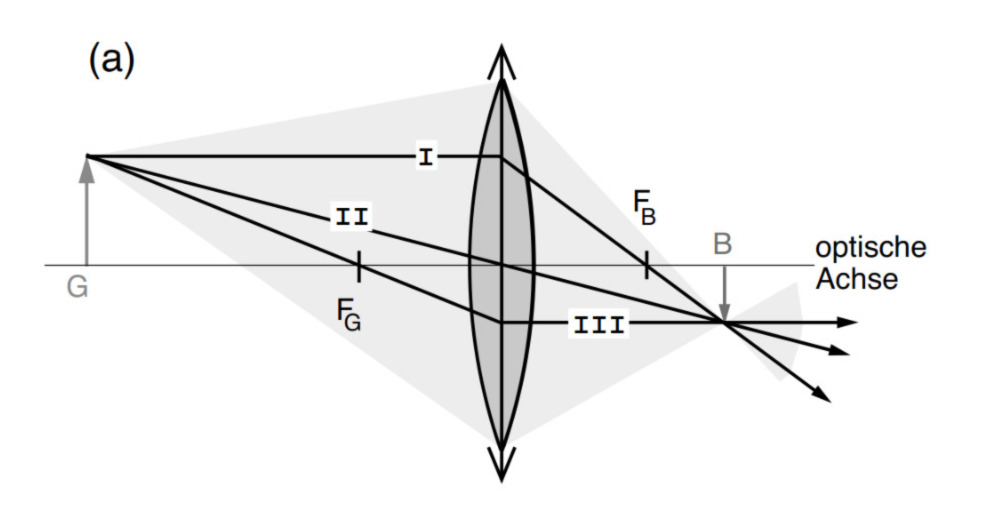
\includegraphics[width=0.5\linewidth]{Abbildungen/Sammellinse.jpeg}
    \caption{
        Bildkonstruktion an einer Sammellinse.
        Quelle: \cite[95]{zinth}
    }
\end{figure}

Die Strahlen (I), (II) und (III) wurden jeweils durch Anwendung der entsprechenden
Regel konstruiert.

\cite[86--97]{zinth}


\subsection{Aufgabe zur Vorbereitung}

In der gesamten Versuchsdurchführung wird jeweils die $H_\alpha$-Linie betrachtet.
Diese entspricht dem Übgergang vom $3$. in den $2$. angeregten Zustand, also
dem Übergang von $n = 2$ zu $m = 3$.

Sei $\lambda_H$ die Wellenlänge der $H_\alpha$-Linie des Wasserstoffatoms
und $\lambda_D$ die der $H_\alpha$-Linie des Deuteriumatoms.
Für das Wasserstoffatom gilt
\[
    \lambda_H \wideeq \left(
        R_H \left( \frac{1}{2^2} - \frac{1}{3^2} \right)
    \right)^{-1}
    \wideeq \frac{m_e + m_H}{m_e m_H} \frac{8 \varepsilon_0^2 h^3 c}{e^4}
    \left( 1/4 - 1/9 \right)^{-1}
    \wideeq \frac{288 (m_e + m_H) \varepsilon_0^2 h^3 c}{5 m_e m_H e^4}
\]
und analog für das Deuteriumatom
\[
    \lambda_D \wideeq \frac{288 (m_e + m_D) \varepsilon_0^2 h^3 c}{5 m_e m_D e^4}.
\]
Daraus berechnet sich eine absolute Wellenlängendifferenz von
\[
    \Delta \lambda
    \wideeq \frac{288 \varepsilon_0^2 h^3 c}{5 e^4}
    \left(
        \frac{m_e + m_H}{m_e m_H} - \frac{m_e + m_D}{m_e m_D}
    \right)
    \wideeq \qty{0.357}{\nm} \quad \coderef{vorbereitung}
\]
sowie eine relative Differenz von
\[
    \frac{\Delta \lambda}{\lambda_H} \wideeq \num{5.44e-4}
    \quad \coderef{vorbereitung}
\]

\newpage

\section{Veruschsablaufplan}

\subsection{Benötigte Materialien}
\subsubsection{Teilversuch 1: Balmer-Serie des Wasserstoffatoms}
    \begin{enumerate}[label=\arabic*.]
        \item H-Lampe
        \item Spaltvorrichtung
        \item Linsen (konkav und konvex gekrümmt)
        \item Reflexionsgitter
        \item CCD-Kamera
        \item Oszilloskop
    \end{enumerate}
\subsubsection{Teilversuch 2: Linienspektrum des Deuteriumatoms}
    \begin{enumerate}[label=\arabic*.]
        \item Spektrallampe ($H_2O+D_2O$-Lampe)
        \item Spaltvorrichtung
        \item 2 Linsen (konvex gekrümmt)
        \item Holografisches Gitter (2400Spalte/mm)
        \item CCD-Kamera
        \item Oszilloskop
    \end{enumerate}

\newpage

\subsection{Teilversuch 1: Balmer-Serie des Wasserstoffatoms}
\begin{enumerate}[label = (\Roman*)]
    \item Ziel: Bestimmen der Rydberg-Konstanten
    
    \item Versuchsmethode: Bestimmen der Wellenlängen der vier sichtbaren Linien der Balmer–Serie des Wasserstoffatoms.
    
    \item Versuchsskizze:
    
        \begin{figure}[H]
        \centering
        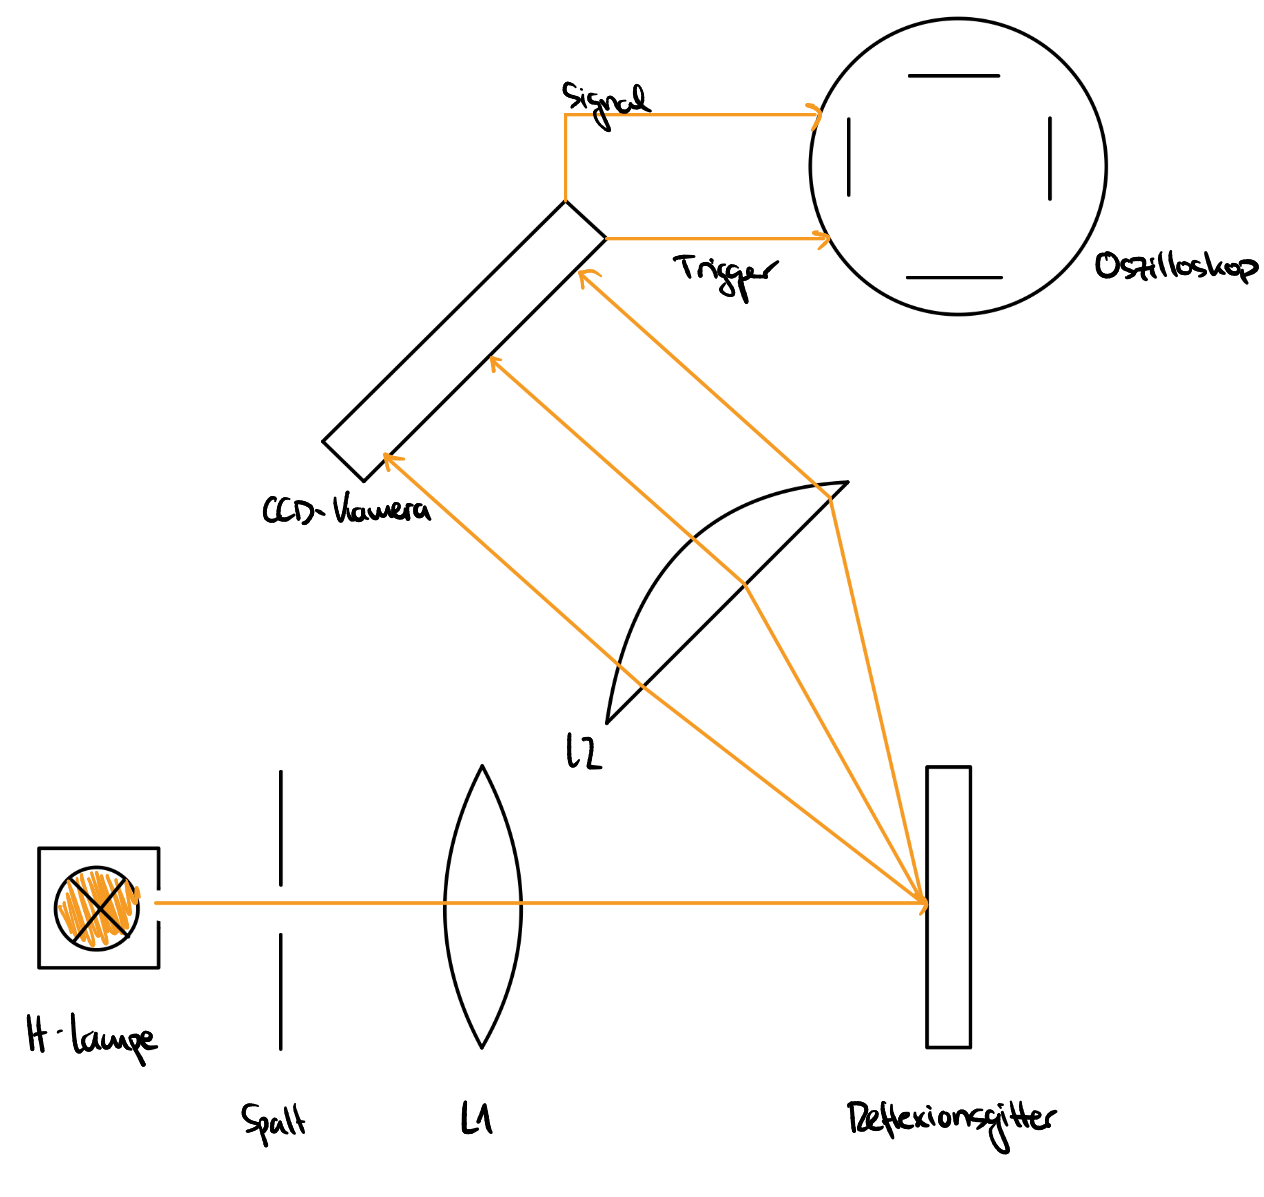
\includegraphics[width=0.7\linewidth]{Abbildungen/TV1.jpeg}
        \caption{Versuchsskizze Teilversuch 1}
        \end{figure}

    \item Planung der Durchführung
        \begin{itemize}
            \item Platzieren der Linse 1 ($f_1=10cm$), damit im Abstand $f$ ein kollimiertes Lichtbündel entsteht
            \item Anpassen des Strahlengangs an die Lochreihe ($h=19cm$)
            \item Gitter so einstellen, dass es senkrecht vom Strahl getroffen wird. Dadurch erreicht man, dass die nullte Ordnung zurückreflektiert wird
            \item Den optischen Tisch so einstellen, dass der Winkel gegen den Nonius 0 Grad beträgt
            \item Suchen der Linien der ersten Ordnung auf einem Schirm hinter dem Versuchsaufbau (Linse 2 $f_2=5cm$)
            \item Spektrum auf CCD-Kamera abbilden
            \item Spektrum am Oszilloskop beobachten und Linsen so justieren, dass alle vier Linien der Balmer-Serie gut sichtbar sind (externe Triggerung der CCD-Kamera)
            \item Aufbau ist nun bereit zur Messung; Raum verdunkeln und mittels Mittelwertfunktion einen möglichst rauscharmen Graph erhalten
            \item Aufnahme stoppen und das erhaltene Spektrum ausdrucken
            \item Mit Hilfe des Cursors alle Positionen der im Spektrum erkennbaren Linien bestimmen (Positionen in Ausdruck notieren)
            \item Wie kann man nun auf die Peaks am CCD schließen?
            \item Verdrehen des Gitters, bis nullte Ordnung auf Bildschirm erscheint
            \item Wieiterdrehen, bis die nullte Ordnung nacheinander mit den Positionen der H-Linien auf dem Bildschirm übereinstimmt. 
            \item Warum abgelesenen Winkel verdoppel?
            \end{itemize}

    \item Vorüberlegungen zur Durchführung \& Auswertung
        \begin{itemize}
            \item Breite der CCD-Zelle: $b=28,75mm$
            \item Winkel immer unter Bezug der Nonius-Skala ablesen
            \item Vergleich mit dem Literaturwert! Wenn sinnvoll: fortfahren, ansonsten Messung wiederholen
            \item Fehlerquellen und Abweichungen!
            \item Woher stammen zusätzliche Linien??
        \end{itemize}
    
\end{enumerate}

\newpage

\subsection{Teilversuch 2: Linienspektrum des Deuteriumatoms}
\begin{enumerate}[label = (\Roman*)]
    \item Ziel: Vergleich des Spektrums des Deuteriumatoms mit dem Spektrum des Wasserstoffatoms 
    
    \item Versuchsmethode: Feststellen einer spektralen Aufspaltung im Wasserstoff–Deuterium-Gemisch
    
    \item Versuchsskizze:
    
        \begin{figure}[H]
        \centering
        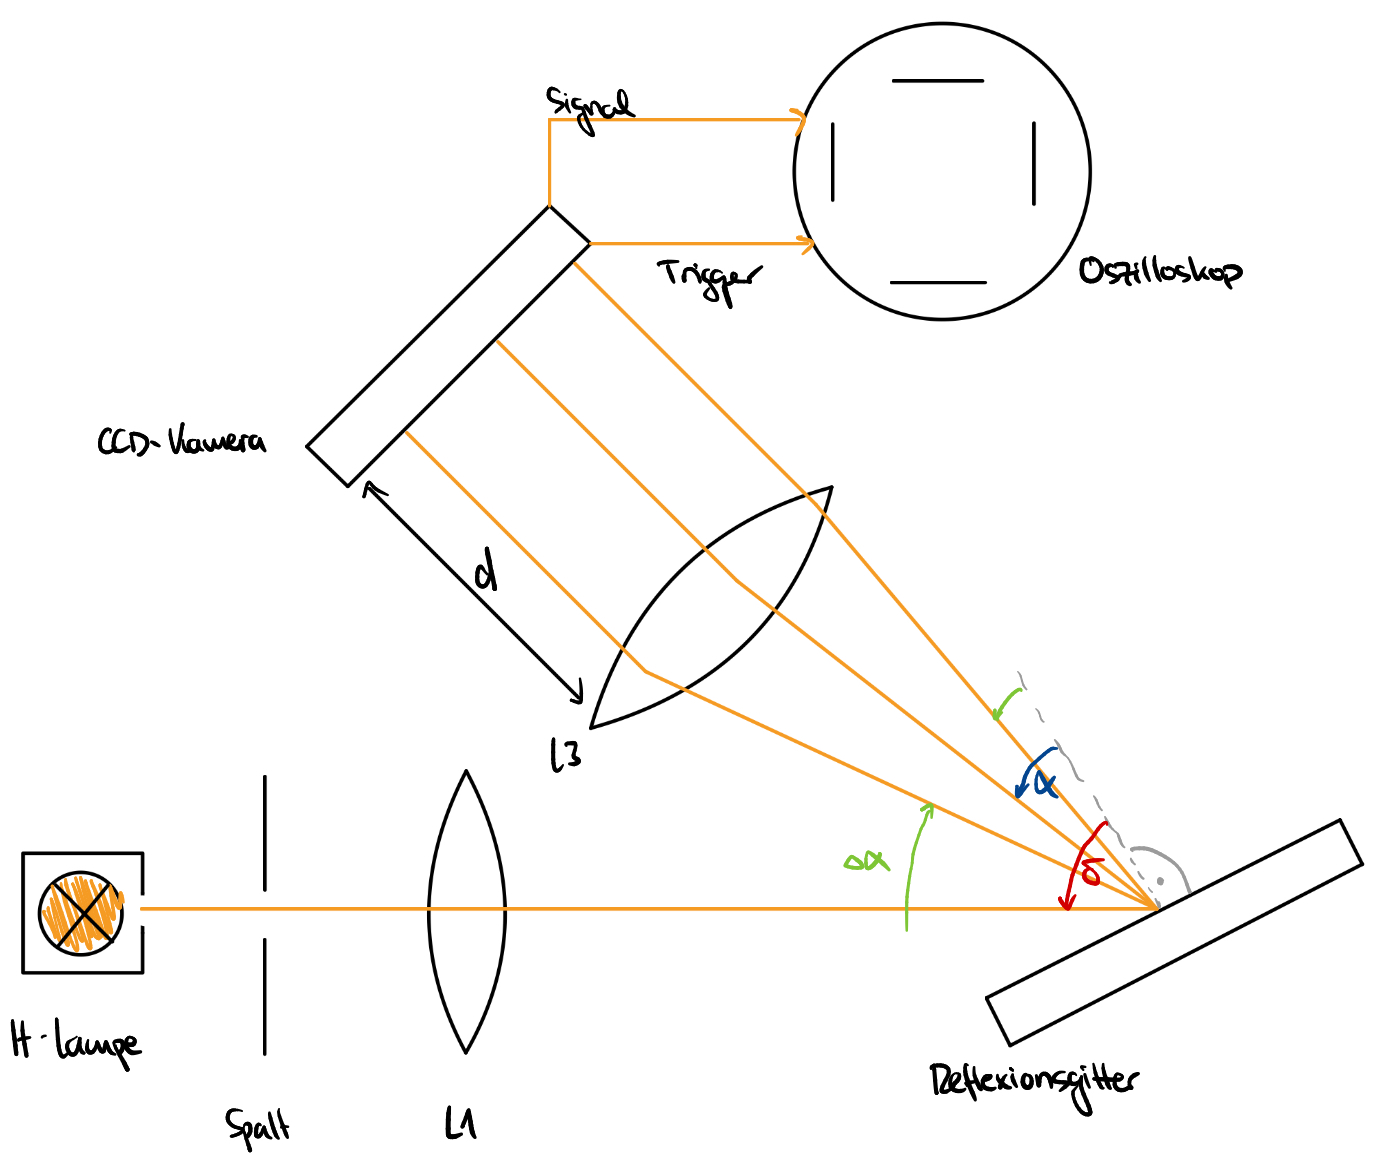
\includegraphics[width=0.7\linewidth]{Abbildungen/TV2.jpeg}
        \caption{Versuchsskizze Teilversuch 2}
        \end{figure}

    \item Planung der Durchführung
        \begin{itemize}
           \item Eine der Balmer-Serien auswählen und mit Hilfe von Linse 3 ($f_3=35cm$) scharf auf CCD-Kamera abbilden
           \item Justieren des Aufbaus, bis eine Aufspaltung der Linien beobachtbar wird
           \item Welches Intesitätsverhältnis ist zu erwarten?
           \item Wellenlängenunterschied bestimmen (Abstand Linse 3 - CCC-Kamera und Linienabstand auf CCD-Kamera messen)
        \end{itemize}

    \item Vorüberlegungen zur Durchführung \& Auswertung
        \begin{itemize}
            \item Warum hat man eine Aufspaltung der Linien? Warum ist diese bei Teilverusch 1 nicht sichtbar?
            \item Wellenlängendifferenz der Doppellinie berechnen
        \end{itemize}
        
\end{enumerate}


\newpage

\iffalse

\section{Versuchsprotokoll}

Auf den folgenden Seiten befindet sich das eingescannte Versuchsprotokoll.
Alle Daten wurden selbst gemessen. Sofern fremde Hilfe benutzt wurde,
wurde sie klar gekennzeichnet.

Messunsicherheiten wurden angegeben und folgend in der Auswertung verwendet.
Alle weiteren Rechnungen und Analysen finden in der Versuchsasuwertung statt.

\includepdf[pages={...}, pagecommand={\thispagestyle{scrheadings}}, frame=true]{[Name.pdf]]}

\newpage

\section{Auswertung}

    \subsection{Teilversuch 1: Bragg-Reflexion von Röntgenstrahlung des Molybdän an einem NaCl-Eiskristall}

\newpage

\fi

\section{Anmerkung: Graphische Auswertung und Fehlerfortpflanzung mit Python-Code}

Alle Berechnungen inkl. Fehlerbestimmung wurden mit einem selbstgeschriebenen
Python-Skript durchgeführt, um uns die Arbeit zu erleichtern und Fehler zu
vermeiden. Alle Ergebnisse, die auf diese Weise zustande gekommen sind,
sind entsprechend mit einem \colorbox{codebg}{blauen Hintergrund} gekennzeichnet;
s. folgendes Beispiel:
\[
    F \wideeq ma \wideeq \qty{20}{\kg} \cdot \qty{9.81}{\meter\per\square\second}
    \wideeq \qty{19.6 \pm 0.5}{\newton} \quad \coderef{tv1}
\]
Dies soll bedeuten, dass die Berechnung des Wertes und der Unsicherheit von der
Python-Funktion namens \verb|tv1| durchgeführt wird.
Die Unsicherheit wird - sofern nicht anders angegeben - mithilfe der Gauß'schen
Fehlerfortpflanzung berechnet.
Außerdem wird das Python-Package \texttt{matplotlib} zum Erstellen
von Graphen verwendet.

Der verwendete Code ist sowohl auf GitHub verfügbar (\githuburl) als auch auf den
folgenden Seiten zu finden und kann mit dem Befehl \texttt{python Main.py}
ausgeführt werden. Für eine genauere Beschreibung des Codes siehe die README-Datei
auf GitHub sowie die Kommentare im Code.
(Manche Sonderzeichen im Code (ä, ö, ü, $\Delta$, etc.) werden von \LaTeX nicht
richtig erkannt, deswegen kann der Code auf den nachfolgenden Seiten an einigen
Stellen unvollständig erscheinen. Auf GitHub wird aber alles richtig angezeigt.)

\newpage


\verb|main.py|:
\lstinputlisting[language=Python]{Code/main.py}
\newpage

% \verb|expressions.py|:
% \lstinputlisting[language=Python]{Code/expressions.py}
% \newpage

Output:
\lstinputlisting{Code/output.txt}

\end{document}